\documentclass{scrartcl}
\usepackage{amsmath,amsfonts,amsthm,bm,graphicx}
\usepackage{tikz,pgfplots}
\usepackage{listings}
\usepackage{stmaryrd}
\usepackage{xcolor}
\usepackage{fdsymbol}
\usepackage{rotating}
\usepackage{listings}
\usepackage{hyperref}

\pgfplotsset{width=15cm,compat=1.18}
\allowdisplaybreaks
\setlength{\parindent}{0pt}

\title{Assignment 2: Modellierung und Differentialgleichungen}
\subtitle{Angewandte Modellierung 25}
\author{Carl Colmant}
\date{\today}
\begin{document}
\maketitle
\newpage
\section*{Exercise 1. Matlab Adventure}
Zuerst soll die Differentialgleichung $30\cos(t) = LI'(t)+ RI(t) = I'(t) + 5I(t)$ gelöst werden mit den Bedingungen $I(0) = 0$. Dazu benutze ich folgenden Matlab Code:\\
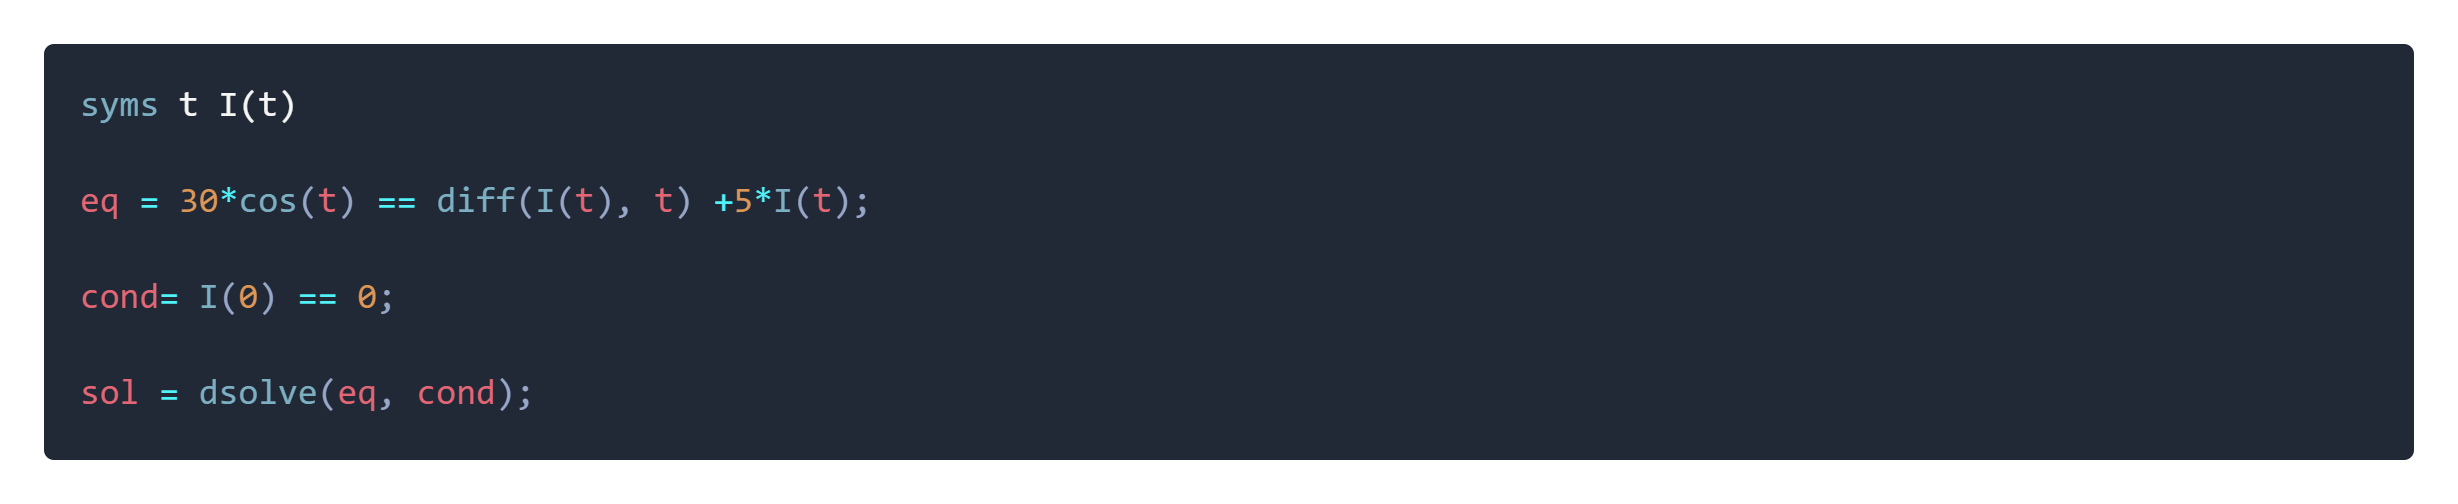
\includegraphics[scale=0.18]{Matlab_adventure.png}\\
Dann soll die Gleichungslösung in punkt $0.5$ ausgewertet werden. Und zu guter letzt die Gleichungslösung über den Zeitbereich $[0, 10]$ dargestellt werden. Dazu benutzte ich folgenden Code:\\
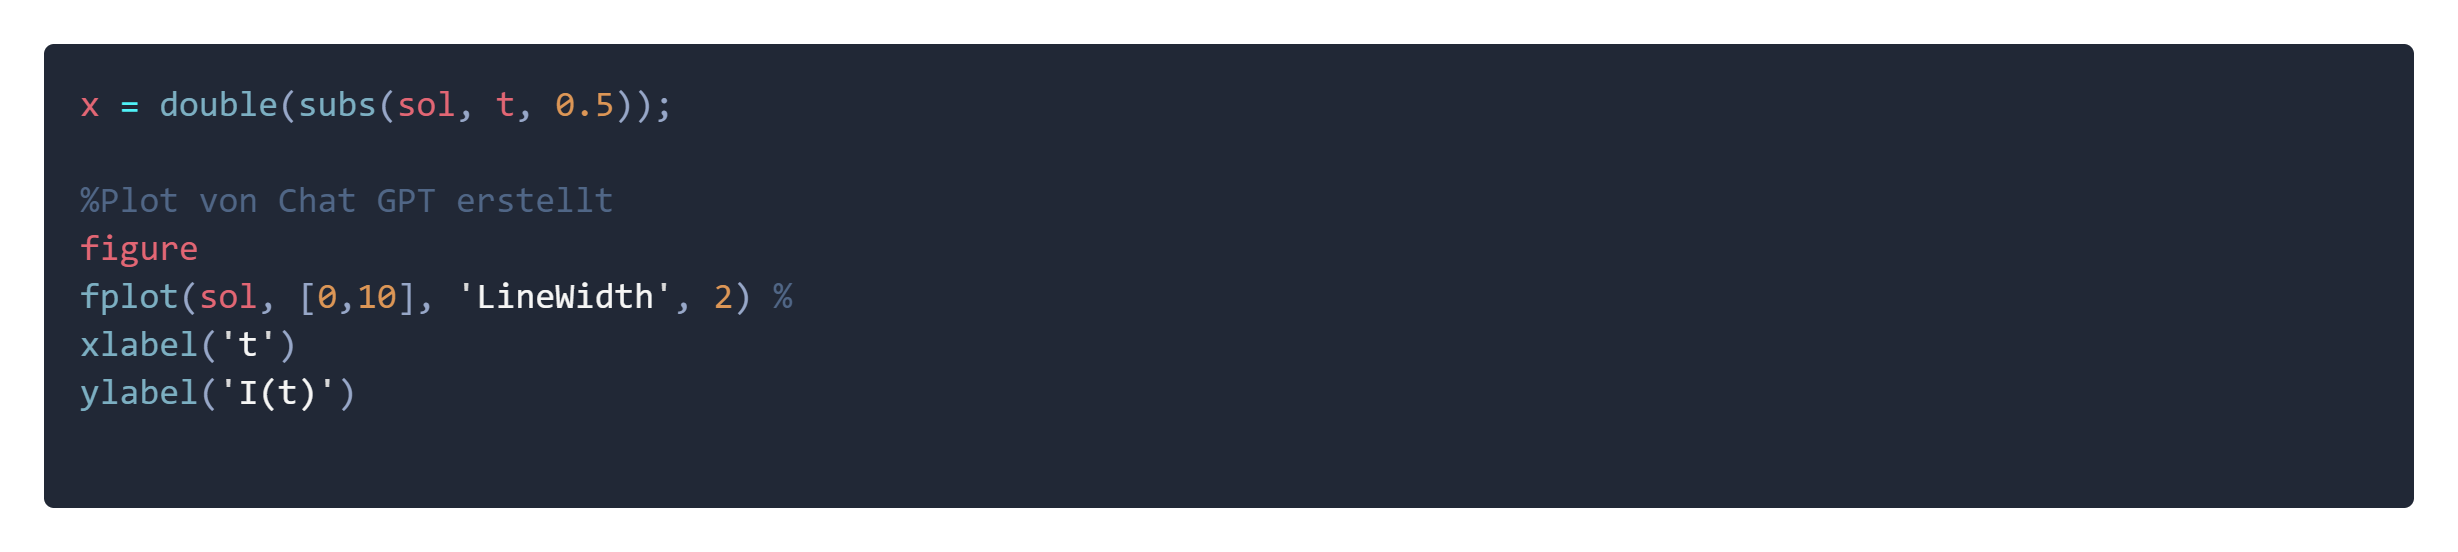
\includegraphics[scale=0.18]{Matlab_adventure2.png}\\


\section*{Exercise 2. Resistor--inductor circuit in Simulink}
Hier sollte ein etwas complexes System aufgebaut werden. Ich hab die Blöcke genau wie in der Aufgabe beschrieben angeordnet den Summenblock mit dem Minuszeichen unten und den Pluszeichen oben ausgestattet. Da kommt dann folgender Graph über 10 sekunden simulationszeit raus:\\
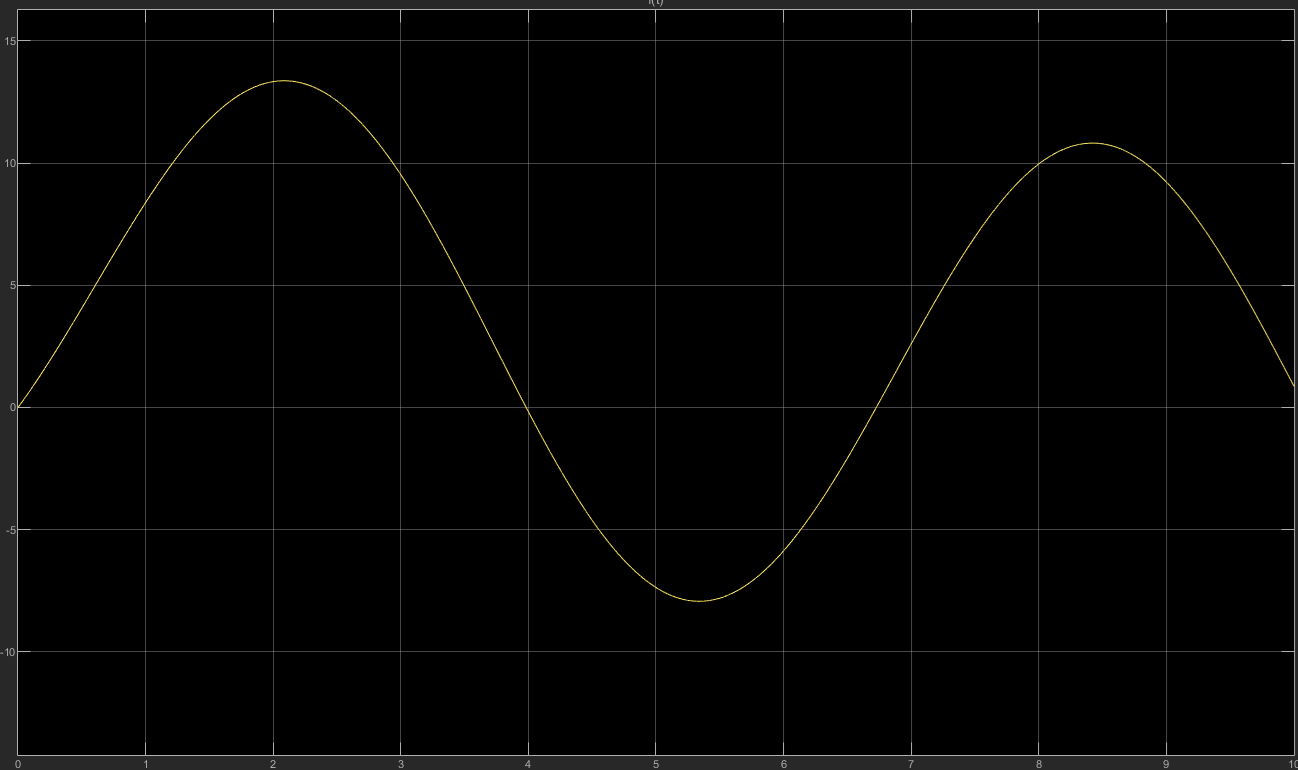
\includegraphics[scale=0.4]{RIC_out.png} 

\section*{Exercise 3. RLC model in Simulink}
Hier ist die Simulation fast identisch aufgebaut, diesmal habe ich aber die Minuszeichen in den Gain-block getan:\\
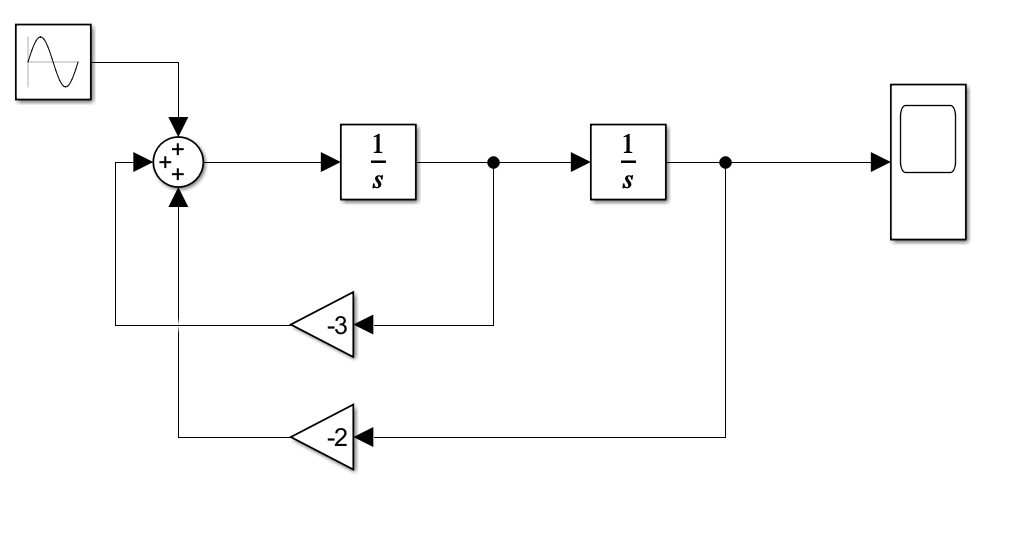
\includegraphics[scale=0.4]{RLC_model.png} \\
Ich habe die Simulation 30 sekunden laufen lassen und das Ergebnis sieht so aus:\\
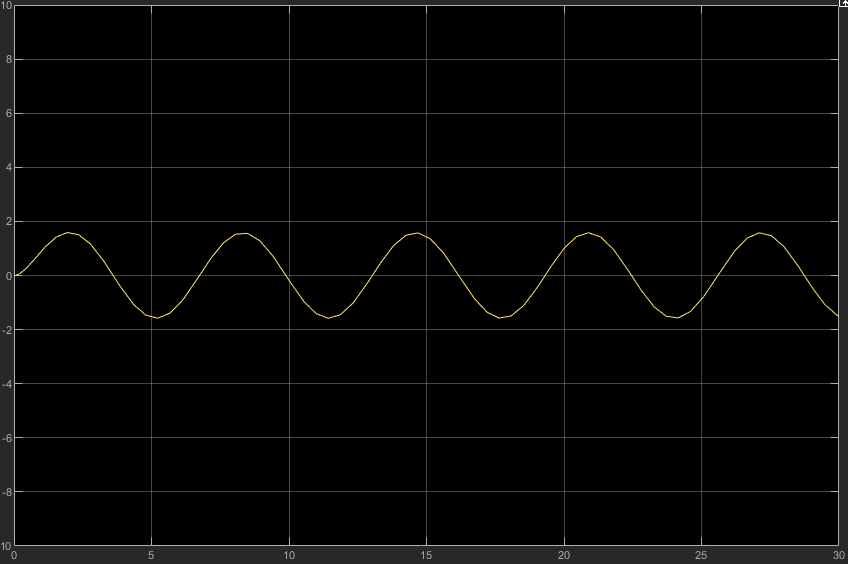
\includegraphics[scale=0.4]{RLC_out.png} \\


\section*{Exercise 4. Fourier series of periodic signals}

Ich habe das Modell so wie in der Aufgabe gezeigt aufgebaut. Man soll die Phase in den Sinus Blöcken auf $\frac{\pi}{2}$ das liegt daran dass die Funktion die approximiert werden soll aus cosinus funktionen besteht. Wenn wir alle Sinus Blöcke korrekt eingestellt haben, lassen wir die Simulation für 920 zeiteinheiten laufen. Es entsteht folgendes Signal:\\
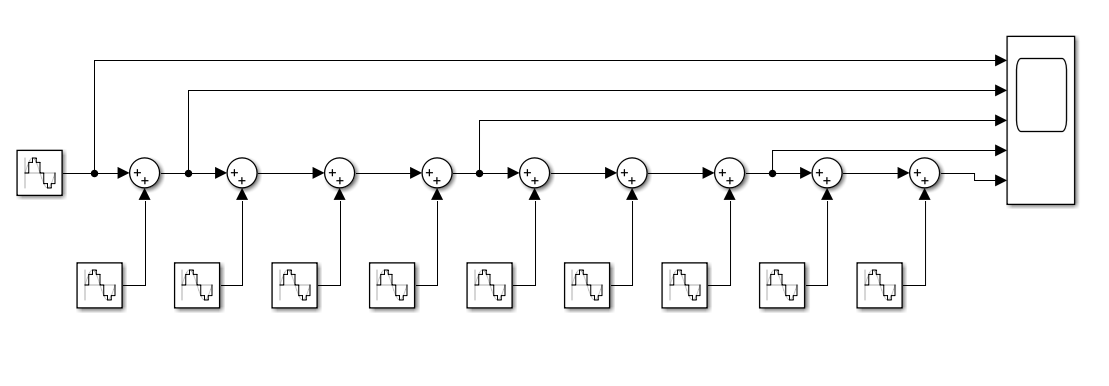
\includegraphics[scale=0.4]{Fourier_modelpng.png} \\
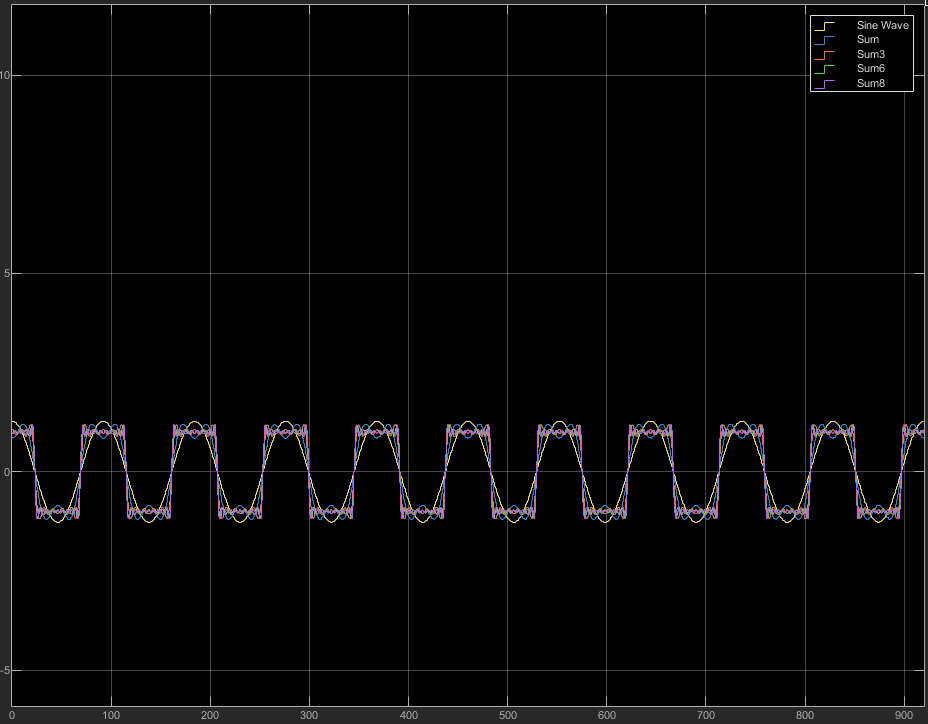
\includegraphics[scale=0.3]{Fourier_out2.png}
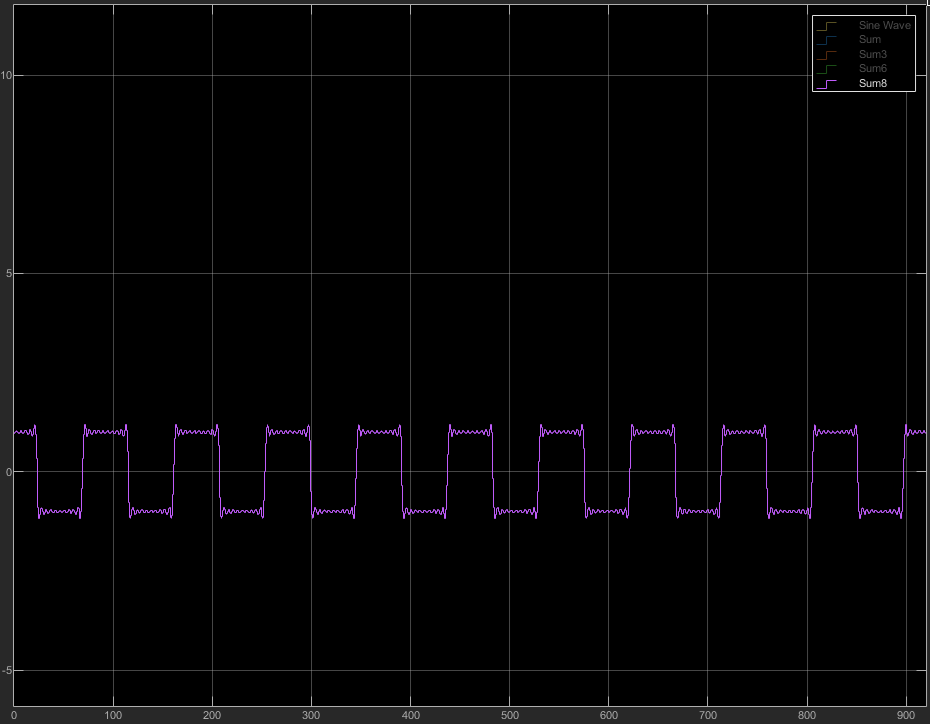
\includegraphics[scale=0.3]{Fourier_out.png} \\

So mehr summen man einbaut desto eckiger und grader wird das Signal. Das heißt die Simulation approximiert die Funktion korrekt.\\

\section*{Exercise 5. Low pass filter}
Wenn man die Funktion die in der Aufgabe aufgeführt ist in Matlab umsetzt erhält man:\\
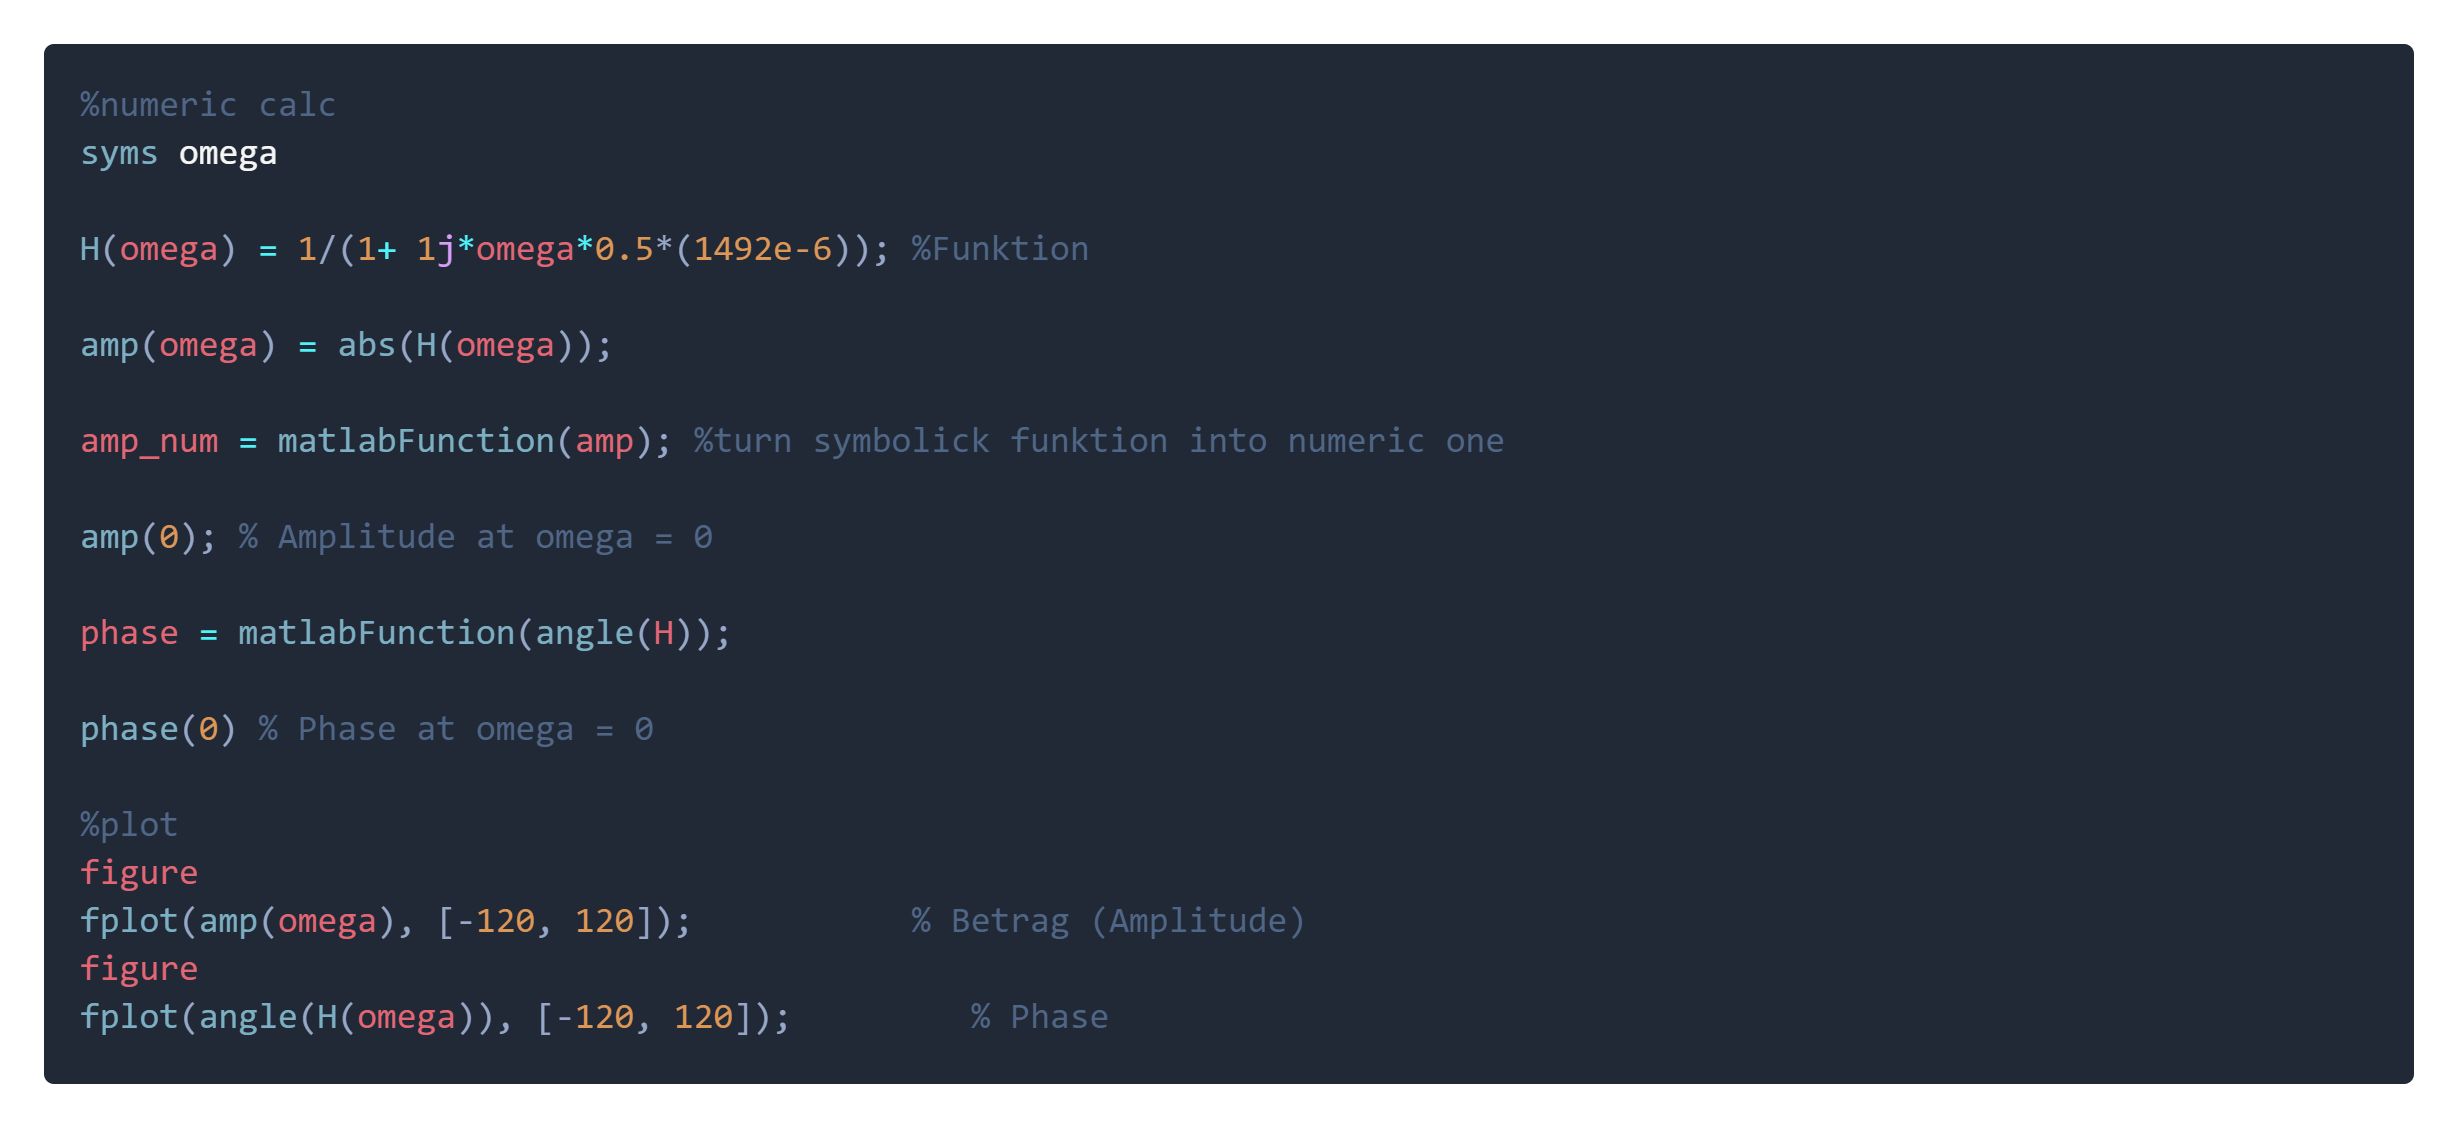
\includegraphics[scale=0.18]{lowpass_filter_code.png}\\
Die Funktion sieht dann so aus:\\
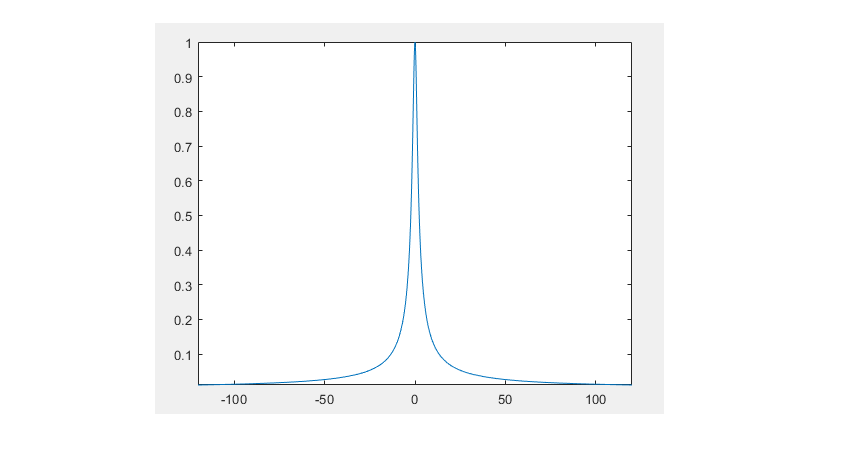
\includegraphics[scale=0.8]{lowpass_filter_out.png}\\
Die Funktion sieht deshalb so aus weil sie die niedrigen Frequenzen unverändert lassen soll (mit 1 multipliziert) und die hohen Frequenzen gedämpft werden sollen(mit <1 multipliziert). Man sieht dass aber noch nicht so gut bei einem so kleinen omega. Hier noch die Phase über omega:\\
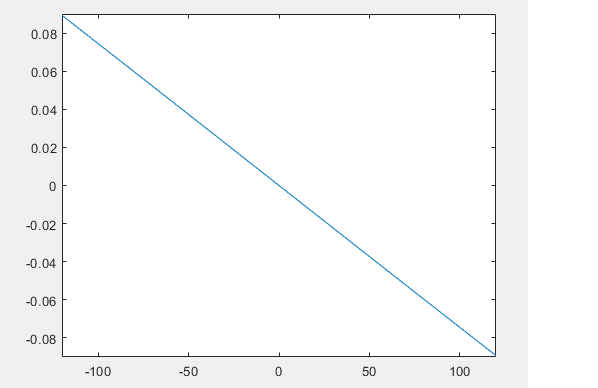
\includegraphics[scale=0.8]{lowpass_filter_out2.png}

 




\end{document}